\documentclass[11pt]{article}
\usepackage{setspace}
\usepackage[a4paper,margin=1in]{geometry}
\geometry{margin=0.85in}
\setstretch{1.0}
\usepackage{graphicx}
\usepackage{array}
\usepackage{setspace}
\usepackage{parskip}
\usepackage{ragged2e}

\pagestyle{empty}
\setstretch{1.05}

\begin{document}


% Title
\begin{center}
    {\Large \textbf{Job Application}} \\[3cm]
    
    {\Huge \textbf{Zhongli Wang}} \\[0.4cm]
    
    {\LARGE Application for Quantitative Researcher}
\end{center}

\vspace{0.6cm}

% Large picture in the middle
\begin{center}
    \IfFileExists{../zhongli-wang-profile.jpg}{
        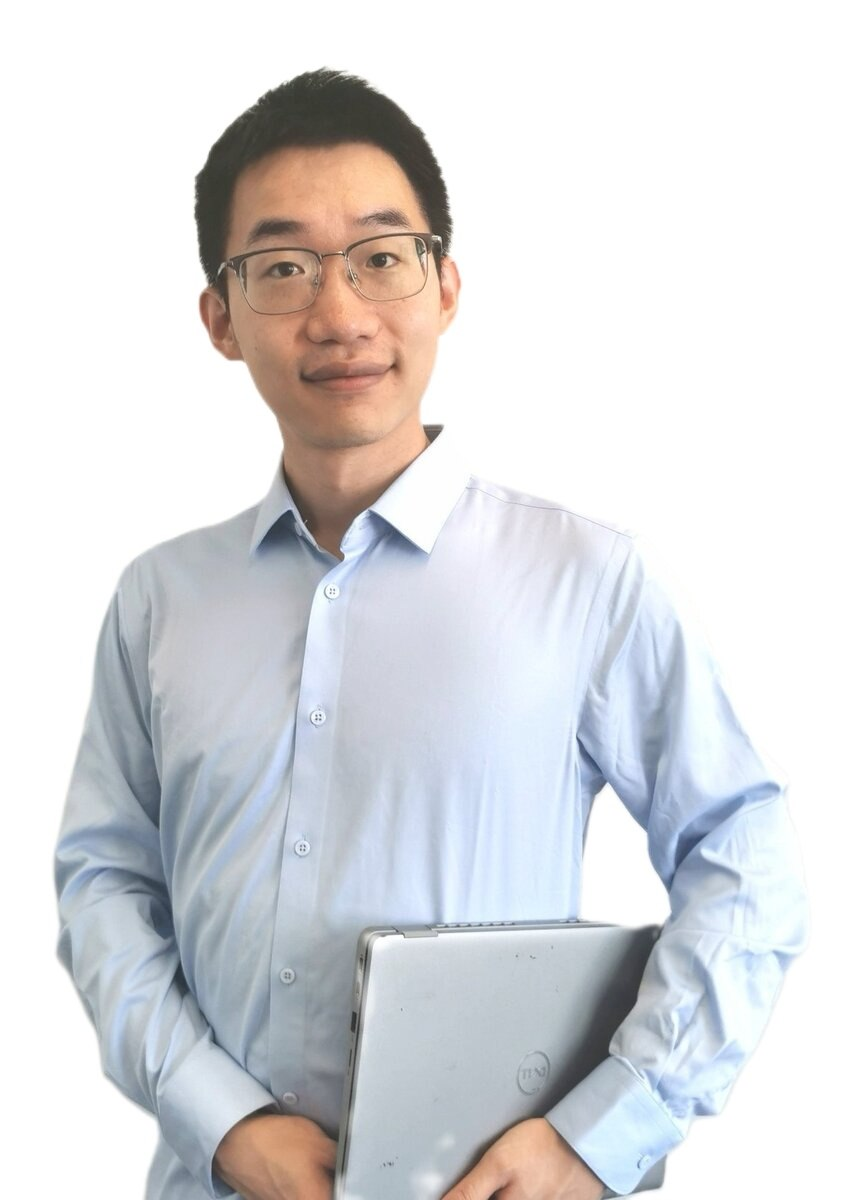
\includegraphics[
            width=0.55\textwidth,
            height=0.45\textheight,
            keepaspectratio
        ]{../zhongli-wang-profile.jpg}
    }{
        \vspace{0.45\textheight}
    }
\end{center}

\vspace{0.7cm}

% \vspace{3cm}


% Personal details
\begin{center}
\renewcommand{\arraystretch}{1.35}
\begin{tabular}{>{\bfseries}p{4.2cm} p{8.5cm}}


Address: & Astastrasse 22, 33617 Bielefeld, Germany \\

Number: & +49 160 9541 6015 \\

Email: & nkwangzhongli@gmail.com \\
\end{tabular}
\end{center}

\vfill

% \begin{center}
%     \small Last updated: \today
% \end{center}
\newpage
\enlargethispage{4\baselineskip}

\begin{flushright}
Zhongli Wang \\
Astastrasse 22 \\
33617 Bielefeld\\
Germany \\
\end{flushright}

\vspace{0.1cm}

\vspace{0.1cm}

\noindent
Jump Trading Group \\
Hong Kong

\vspace{0.12cm}

\noindent
\textbf{Application for Quantitative Researcher}

\vspace{0.1cm}

\noindent Dear Jump Trading recruiting team,

I am completing a Ph.D. in Economics at Bielefeld University, with my defense scheduled for September 21, 2026, 
and I hold an M.A. in Business and Economics with a major in Banking and Finance and a minor in Data Science, as well as a B.Sc. in Finance. 
My research combines statistical modeling, machine learning, Python-based computational work, and financial data analysis. 
I am applying for the Quantitative Researcher role because the team requires exactly the disciplined empirical approach I bring: 
collecting noisy data, forming testable hypotheses, building forecasts, and converting validated signals into predictive models.

I am particularly drawn to Jump because the role sits at the intersection of scientific research, 
machine learning, data engineering, and global financial markets. 
Your posting emphasizes creativity, intellectual honesty, collaboration, and a competitive research culture. 
That matches how I work: I build models from explicit assumptions, test them against data, inspect failures, 
and communicate results clearly enough for others to challenge or extend.
My relevant experience comprises:

\begin{itemize}
    \item \textbf{Forecasting and machine learning:} In a published financial fraud detection project, I applied XGBoost and Random Forest to accounting, financial, and market indicators from listed companies. This trained me to evaluate predictive features and separate robust signals from noisy correlations.
    \item \textbf{Quantitative research discipline:} My doctoral work develops computational models of strategic firm behavior under uncertainty. I estimate parameters, test model mechanisms, and analyze how market structure, capacity limits, and network effects change outcomes.
    \item \textbf{Programming and data work:} I use Python extensively for computational modeling, machine learning, and data analysis, with additional experience in R, Julia, Mathematica, SQL, Git, and Linux-based workflows.
    % \item \textbf{Communication and drafting:} I have authored peer-reviewed publications, prepared technical reports, and presented complex economic arguments at international conferences. I have strong drafting skills in both English and German, with experience translating technical analysis into accessible insights for diverse audiences.
\end{itemize}

I have excellent command of both German and English at C1 level, and I am a native Mandarin Chinese speaker. 
I am open to Hong Kong as a long-term location and would value the chance to contribute to a team that combines quantitative research, ML/LLM expertise, and engineering in one research process. 
My academic training is aligned with the analytical core of the role: 
statistical inference, financial data, machine learning, programming, and careful model validation. 
At Jump, I would aim to contribute through clean research pipelines, rigorous forecast evaluation, and empirical work that is direct about uncertainty.

Thank you so much for considering my application! 
I would welcome the opportunity to discuss how my research background, financial training, and coding experience could contribute to Jump's quantitative research team in Hong Kong.

\vspace{0.08cm}
\noindent Kind regards, \\
\noindent Zhongli Wang

\vspace{0.1cm}
\noindent
\includegraphics[width=2.7cm,keepaspectratio]{../Wang-sig.jpg}

\end{document}
